\documentclass[11pt,a4paper]{article}
\usepackage[margin=2.4cm]{geometry}
\usepackage{amsmath,amssymb,bm}
\usepackage{booktabs,array}
\usepackage{graphicx}
\usepackage{microtype}
\usepackage{xcolor}
\usepackage{fancyhdr}
\usepackage[colorlinks=true,linkcolor=blue!50!black,urlcolor=blue!50!black]{hyperref}
\setlength{\parindent}{0pt}
\setlength{\parskip}{0.55em}
\pagestyle{fancy}\fancyhf{}
\lhead{Physics of the Shape Analytics simulators}\rhead{\thepage}
\renewcommand{\headrulewidth}{0.3pt}
\newcommand{\tens}[1]{\bm{#1}}
\newcommand{\app}[1]{\par\smallskip\noindent\textbf{In the app.} #1}
\newcommand{\sig}[1]{\par\smallskip\noindent\textbf{Physical significance.} #1}

\title{Physical Significance and Governing Principles\\of the Shape Analytics Simulators}
\author{Course project, Mechanics of Solids}
\date{\today}

\begin{document}
\maketitle
\tableofcontents
\newpage

\section{Purpose and structure}
The Shape Analytics app is a suite of interactive solid mechanics simulators. Its aim is to make stress analysis \emph{move}: the user changes a load, a geometry or a material and sees the stress state, the deformation and the safety margin respond immediately. Every simulator is tied to one or more chapters of the course notes (Chapters 1 to 11). This report states, chapter by chapter, the principle used, the equations implemented, and what the quantity means physically.

Each simulator provides the same features: a live diagram, analytic charts, an A/B comparison (a saved baseline is overlaid on every chart), and exports (CSV, SVG, PNG, a design specification, and a lab report). All inputs use N, mm and MPa unless the label says otherwise.

\begin{table}[h]
\centering
\begin{tabular}{@{}p{3.6cm}p{3.1cm}p{7.3cm}@{}}
\toprule
Simulator & Chapters & Main principle used\\
\midrule
3D stress field & 2, 3, 4, 5, 6 & Cauchy's theorem, equilibrium, strain--displacement, Hooke's law, half-space (Boussinesq, Cerruti) solution\\
Mohr's circle & 1, 2, 4 & Tensor transformation, principal values, invariants, hydrostatic/deviatoric split\\
Beam analysis & 3, 8, 9 & Equilibrium, pure and non-uniform bending, Euler--Bernoulli and Timoshenko theory\\
Shaft torsion & 7 & Axisymmetric equilibrium and compatibility for twist\\
Axial loading & 6, 7 & Extension of a bar, superposition, thermoelastic strain\\
Pressure vessel & 7 & Inflation of a cylinder, Lam\'e solution\\
Thermal stress & 6 & Isotropic thermoelasticity\\
Failure theories & 11 & Maximum principal stress, strain, shear and distortional energy criteria\\
Energy methods & 10 & Strain energy, reciprocity, Castigliano's theorem\\
Column buckling & 9 & Euler buckling, effective length\\
\bottomrule
\end{tabular}
\caption{Simulators and the chapters they implement.}
\end{table}

\section{Chapter 1: Mathematical preliminaries}
Stress and strain are second-order tensors. A tensor is a physical object that exists independent of coordinates; a matrix is its representation in one basis. For a rotation tensor $\tens{Q}$ the components change as $[\tens{T}]' = \tens{Q}[\tens{T}]\tens{Q}^{T}$, while scalar combinations such as the trace and determinant do not.

\sig{This is why Mohr's circle and the invariants are meaningful. The material does not care how an analyst chose the axes, so any failure rule must depend only on quantities that survive rotation.}
\app{The Mohr's circle simulator applies $\tens{Q}$ about $z$ to the stress matrix and reports the rotated components next to the invariants.}

\section{Chapter 2: Traction vector and stress tensor}
\subsection{Traction}
Cutting a body along a plane with outward unit normal $\tens{n}$ exposes a distributed force. The traction is the force per unit area,
\begin{equation}
\tens{t}(\tens{x};\tens{n}) = \lim_{\Delta A\to 0}\frac{\Delta\tens{F}}{\Delta A}.
\end{equation}
Applying linear momentum balance to an infinitesimal tetrahedron, the body force and inertia terms scale with volume ($h^3$) and vanish faster than the surface terms ($h^2$). What remains is Cauchy's theorem,
\begin{equation}
\tens{t}_n = \tens{\sigma}\,\tens{n},\qquad
\tens{\sigma}=\sum_{i}\tens{t}_i\otimes\tens{e}_i .
\end{equation}
\sig{Traction on every plane through a point is fixed by just three vectors (nine numbers). Normal traction $\sigma_n=\tens{n}\cdot\tens{\sigma}\tens{n}$ pulls or pushes the planes apart; the in-plane part $\tau$ slides them. Stress is therefore local force transmission, not a property of a particular plane.}

\subsection{Transformation}
Under rotation of axes the stress matrix transforms as $[\tens{\sigma}]'=\tens{Q}[\tens{\sigma}]\tens{Q}^T$. For plane stress rotated by $\theta$,
\begin{align}
\sigma_{x'} &= \tfrac{\sigma_x+\sigma_y}{2}+\tfrac{\sigma_x-\sigma_y}{2}\cos2\theta+\tau_{xy}\sin2\theta,\\
\tau_{x'y'} &= -\tfrac{\sigma_x-\sigma_y}{2}\sin2\theta+\tau_{xy}\cos2\theta .
\end{align}
\app{In the 3D stress field the applied traction on a painted area is decomposed into normal and shear parts using exactly $\sigma_n=\tens{t}\cdot\tens{n}$ and $\tens{t}_s=\tens{t}-\sigma_n\tens{n}$. The Mohr's circle simulator implements the transformation above.}

\section{Chapter 3: Stress equilibrium equations}
Linear momentum balance for a small element gives
\begin{equation}
\nabla\cdot\tens{\sigma}+\rho\tens{b}=\rho\ddot{\tens{u}},
\end{equation}
and angular momentum balance, in the absence of body couples, gives $\tens{\sigma}=\tens{\sigma}^T$ (so $\tau_{xy}=\tau_{yx}$ and so on). The traction boundary condition is $\tens{\sigma}\tens{n}=\bar{\tens{t}}$ on the loaded surface.

\sig{Equilibrium says that stress cannot be chosen freely: its gradient must balance the body force, which is why stress varies smoothly through a loaded body. Symmetry of $\tens{\sigma}$ means a pair of shear stresses always acts on perpendicular faces, so six independent components suffice.}
\app{The beam simulator uses the integrated form of equilibrium, $dV/dx=-w$ and $dM/dx=V$, to draw the shear-force and bending-moment diagrams. The mohr simulator accepts only symmetric shears for the same reason.}

\section{Chapter 4: Principal values, maximum shear and Mohr's circle}
Principal planes are the planes on which traction is purely normal, so $\tens{\sigma}\tens{n}=\lambda\tens{n}$. They solve the eigenvalue problem
\begin{equation}
\lambda^3-I_1\lambda^2+I_2\lambda-I_3=0,
\end{equation}
with the invariants
\begin{equation}
I_1=\operatorname{tr}\tens{\sigma},\quad
I_2=\sigma_x\sigma_y+\sigma_y\sigma_z+\sigma_z\sigma_x-\tau_{xy}^2-\tau_{yz}^2-\tau_{zx}^2,\quad
I_3=\det\tens{\sigma}.
\end{equation}
The roots are real, the principal directions are orthogonal, and the principal stresses are the extreme values of the normal traction. The maximum shear stress is $\tau_{\max}=(\sigma_1-\sigma_3)/2$ on planes at $45^\circ$ to the extreme principal directions. In the $(\sigma,\tau)$ plane the state of every plane lies on or between three circles, with diameters $\sigma_1-\sigma_3$, $\sigma_1-\sigma_2$ and $\sigma_2-\sigma_3$ (Mohr's circle and Mohr's stress plane). The stress splits into a hydrostatic part $p\tens{I}$ with $p=I_1/3$ (volume change) and a deviatoric part $\tens{s}=\tens{\sigma}-p\tens{I}$ (shape change).

\sig{Principal stresses are the largest and smallest tensile or compressive intensities a point feels, and they decide where a brittle material cracks. The maximum shear controls ductile slip. The hydrostatic part changes volume but not shape, and the deviatoric part changes shape; this separation reappears in the von Mises criterion.}
\app{The simulator solves the cubic with the trigonometric (Lode) form, draws the three circles, marks the rotating face as a point that moves twice as fast as the element, and reports $I_1,I_2,I_3$, $p$ and the failure margin.}

\begin{figure}[h]
\centering
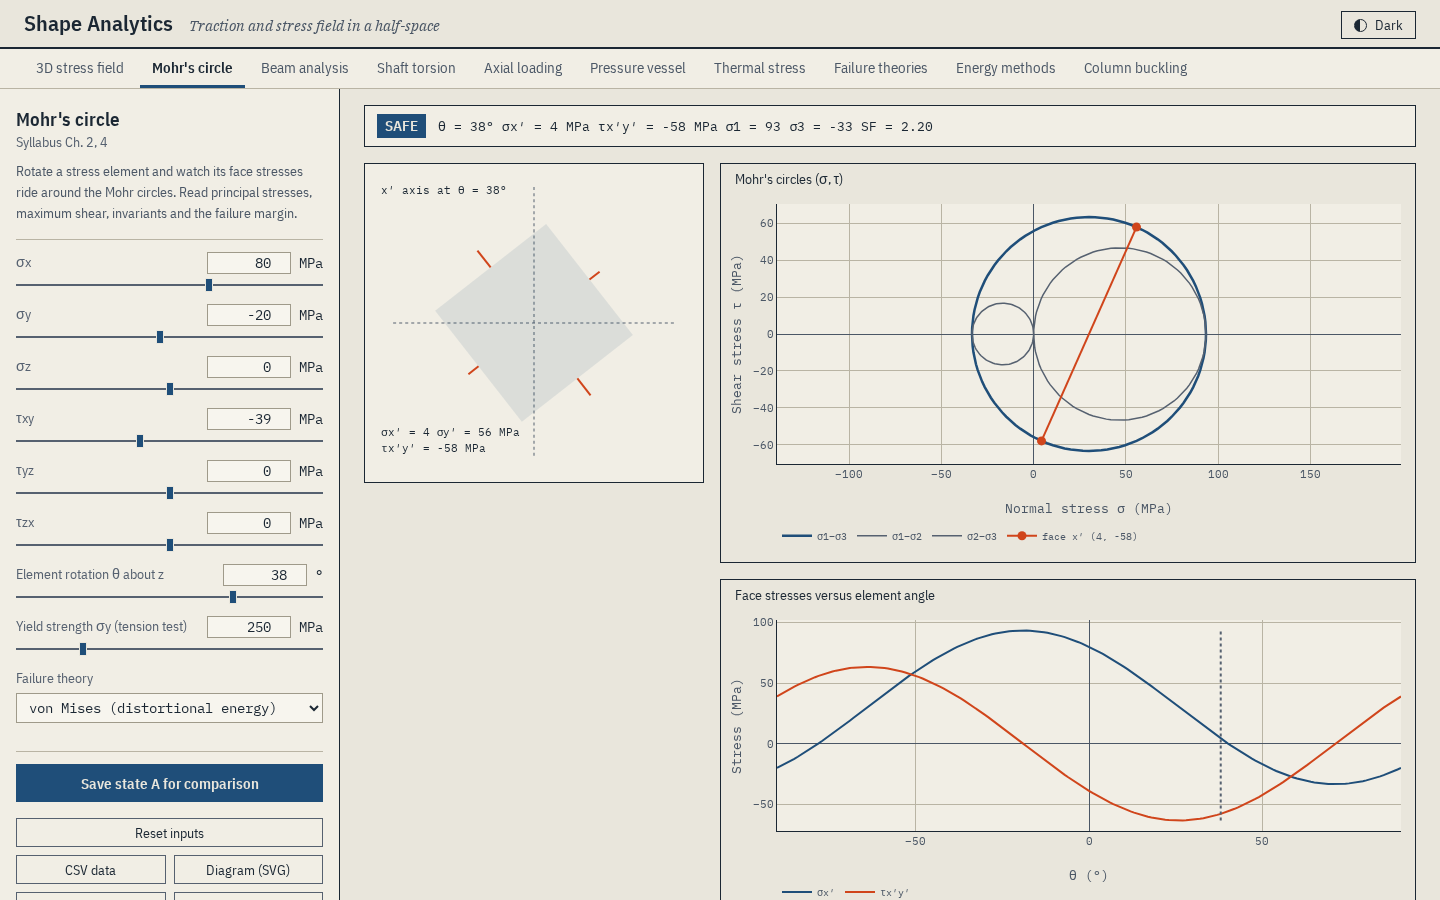
\includegraphics[width=\linewidth]{figures/mohr.png}
\caption{Mohr's circle simulator: the rotated element, the three circles and the face stresses versus angle.}
\end{figure}

\section{Chapter 5: Strain tensor}
Deformation is described by mapping a reference configuration to a deformed one. For small deformation the strain tensor is the symmetric part of the displacement gradient,
\begin{equation}
\tens{\varepsilon}=\tfrac12\left(\nabla\tens{u}+\nabla\tens{u}^T\right),
\end{equation}
with longitudinal strain $\varepsilon_{xx}=\partial u_x/\partial x$, shear strain $\gamma_{xy}=2\varepsilon_{xy}$, and volumetric strain $\varepsilon_v=\operatorname{tr}\tens{\varepsilon}$. The antisymmetric part is a local rigid rotation. Six strain components derive from three displacements, so they must satisfy compatibility conditions or the body would tear or overlap. Strain transforms exactly like stress, so there are principal strains and a Mohr's circle for strain.

\sig{Strain measures how much neighbouring points move relative to each other, after removing rigid motion. It is the quantity the material actually responds to, which is why constitutive laws link stress and strain.}
\app{The 3D stress field colours the body by strain magnitude and exaggerates the displacement field computed from the half-space solution so the deformed shape is visible. Axial, torsion and thermal simulators compute normal, shear and thermal strain respectively.}

\section{Chapter 6: Stress--strain relations}
A linear elastic solid obeys $\sigma_{ij}=C_{ijkl}\varepsilon_{kl}$. Symmetry of stress, strain and of the strain energy reduces the 81 constants to 21 for the most general material and to two for an isotropic one,
\begin{equation}
\sigma_{ij}=\lambda\,\varepsilon_{kk}\delta_{ij}+2\mu\,\varepsilon_{ij},\qquad
\varepsilon_{ij}=\tfrac{1+\nu}{E}\sigma_{ij}-\tfrac{\nu}{E}\sigma_{kk}\delta_{ij}.
\end{equation}
The engineering constants are related by $G=\mu=E/2(1+\nu)$ and $K=E/3(1-2\nu)$. With a temperature change the free strain $\alpha\Delta T\,\delta_{ij}$ is added, giving isotropic thermoelasticity $\varepsilon_{ij}=\frac{1+\nu}{E}\sigma_{ij}-\frac{\nu}{E}\sigma_{kk}\delta_{ij}+\alpha\Delta T\delta_{ij}$.

\sig{$E$ is stiffness in tension, $G$ is stiffness in shear, $\nu$ is the sideways contraction that accompanies stretching, and $K$ is resistance to volume change. Heating produces strain without stress; stress appears only if the supports prevent the strain.}
\app{The material selector fixes $E$, $\nu$, $\alpha$ and $\sigma_y$ for every simulator and the readouts show $G$ and $K$. The thermal stress simulator implements the constrained cases
\begin{equation}
\sigma_{\text{bar}}=-E\alpha\Delta T,\quad
\sigma_{\text{plate}}=\frac{-E\alpha\Delta T}{1-\nu},\quad
\sigma_{\text{block}}=\frac{-E\alpha\Delta T}{1-2\nu}.
\end{equation}
The more directions are blocked, the stiffer the effective response and the larger the stress.}

\section{Chapter 7: Axisymmetric problems}
In cylindrical coordinates $(r,\theta,z)$ the equilibrium equation in the radial direction reads $\frac{d\sigma_{rr}}{dr}+\frac{\sigma_{rr}-\sigma_{\theta\theta}}{r}=0$ when the fields depend on $r$ only. The chapter solves three canonical problems for a long cylinder: extension, torsion and inflation.

\subsection{Extension and torsion}
For extension, $\sigma_{zz}=N/A$ and $\delta=NL/EA$. For torsion, physical symmetry says plane sections stay plane and rotate rigidly, so $\gamma_{\theta z}=r\,d\phi/dz$ and, from Hooke's law,
\begin{equation}
\tau(r)=\frac{T r}{J},\qquad J=\frac{\pi}{32}(D^4-d^4),\qquad \phi=\frac{TL}{GJ}.
\end{equation}
\sig{Torque is carried only by shear stress that grows linearly with radius, so material near the axis is under-used and a hollow shaft keeps most of the stiffness at much lower mass. Torsional stiffness $GJ/L$ plays the same role for twist that $EA/L$ plays for stretch.}
\app{The axial simulator handles stepped bars in series, a fixed--fixed redundant case by compatibility $\sum\delta_i=0$, and thermal strain. The torsion simulator plots $\tau(r)$ and $\phi(x)$ and compares the stiffness of the hollow and solid sections.}

\subsection{Inflation of a cylinder (Lam\'e)}
Equilibrium plus Hooke's law plus compatibility give $\sigma_{rr}=A-B/r^2$ and $\sigma_{\theta\theta}=A+B/r^2$. The boundary conditions $\sigma_{rr}(a)=-p_i$ and $\sigma_{rr}(b)=-p_o$ fix
\begin{equation}
A=\frac{p_ia^2-p_ob^2}{b^2-a^2},\qquad
B=\frac{(p_i-p_o)a^2b^2}{b^2-a^2},
\end{equation}
and, for closed ends, $\sigma_{zz}=A$. For thin walls this reduces to $\sigma_\theta=pr/t$ and $\sigma_z=pr/2t$; for a sphere $\sigma_\theta=\sigma_\phi=pr/2t$.

\sig{Internal pressure tries to enlarge the vessel, and the wall resists with hoop tension, exactly as a hoop around a barrel does. The hoop stress is twice the axial stress, so a pressurised cylinder splits along its length. In a thick wall the hoop stress is largest at the inner surface, where the radial stress also equals $-p_i$.}

\begin{figure}[h]
\centering
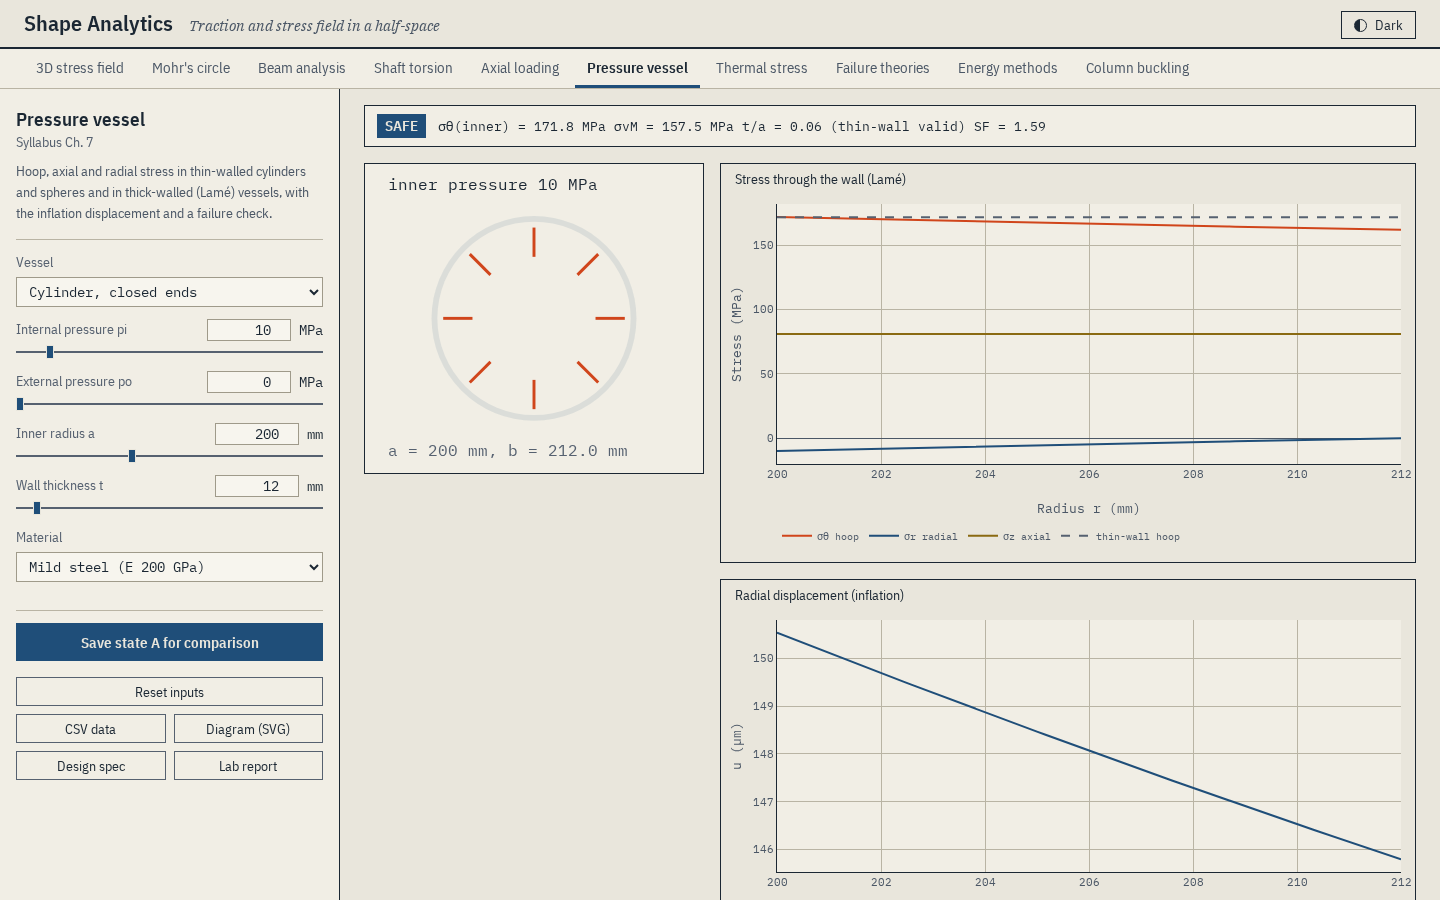
\includegraphics[width=0.92\linewidth]{figures/pressure.png}
\caption{Pressure vessel simulator: Lam\'e stresses through the wall with the thin-wall hoop stress for comparison.}
\end{figure}

\section{Chapter 8: Bending of beams}
\textbf{Pure bending.} Plane sections remain plane and normal to the axis, so axial strain varies linearly with distance $y$ from the neutral axis. With zero net axial force the neutral axis passes through the centroid, and
\begin{equation}
\sigma_{xx}=-\frac{My}{I},\qquad \frac{1}{\rho}=\frac{M}{EI}.
\end{equation}
\textbf{Non-uniform bending.} When the moment varies, the shear force $V=dM/dx$ produces shear stress
\begin{equation}
\tau=\frac{VQ}{Ib},\qquad Q=\int_{y}^{c}y'\,b(y')\,dy',
\end{equation}
which is largest at the neutral axis (for a rectangle $1.5V/A$, for a solid circle $4V/3A$). Unsymmetrical sections need the product of inertia and a shear centre, the point through which the load must act to avoid twist.

\sig{The beam carries load by stretching one side and shortening the other, so fibres far from the neutral axis do the work, which is why deep or I-shaped sections are efficient. Shear is carried by the web, and the shear stress is zero at the outer surface.}
\app{The beam simulator solves statics for simply supported and cantilever beams under a point load, a uniform load and an applied moment, then integrates the curvature numerically. It plots $V$, $M$, deflection, and the through-depth distributions of $\sigma$ and $\tau$ for rectangular, solid and hollow circular sections.}

\begin{figure}[h]
\centering
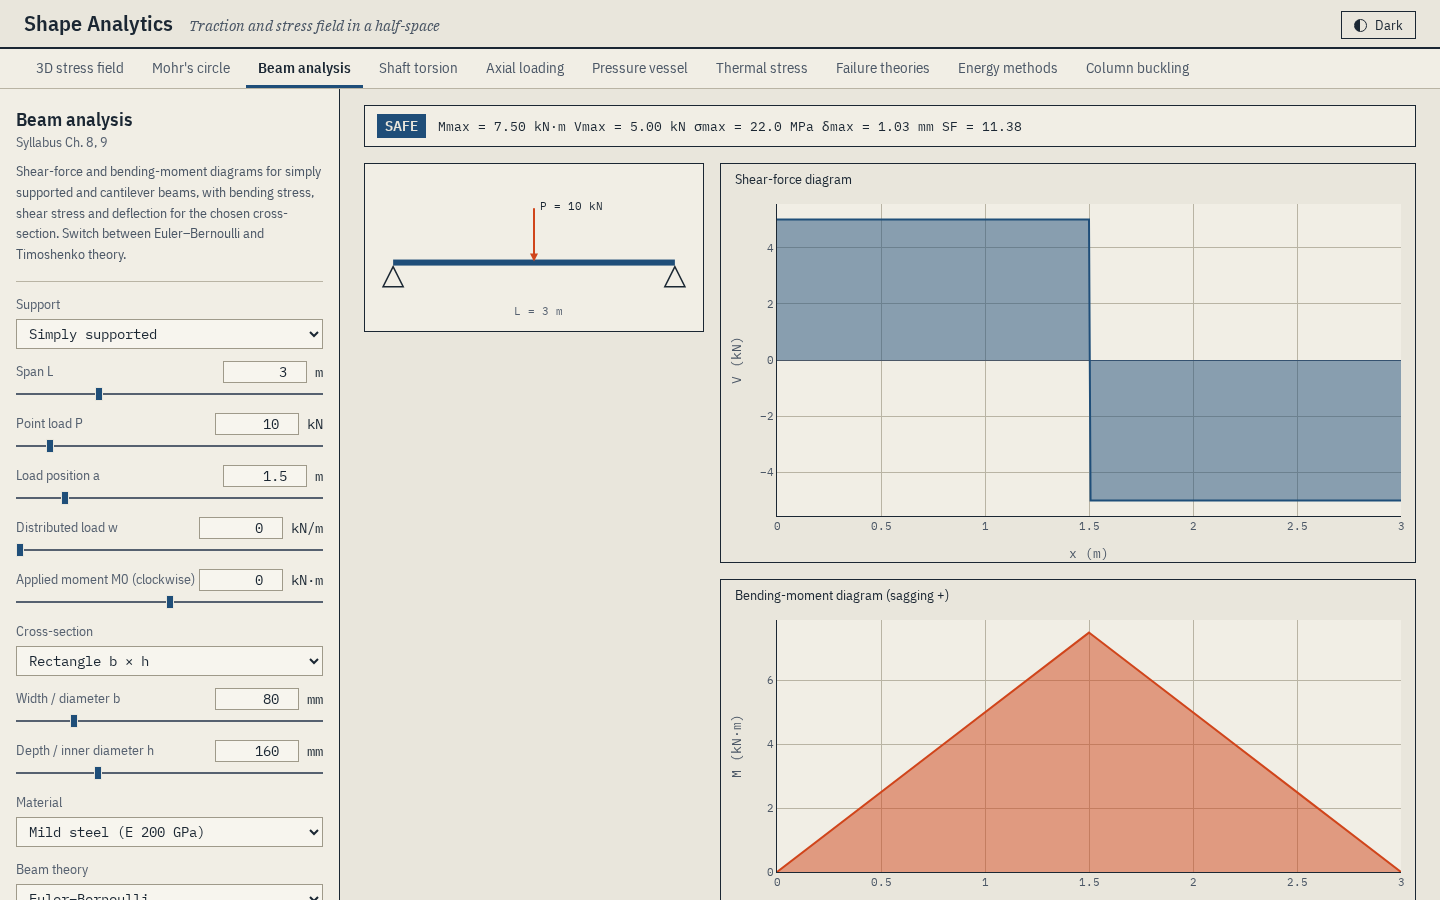
\includegraphics[width=\linewidth]{figures/beam.png}
\caption{Beam simulator: loading diagram, shear force and bending moment.}
\end{figure}

\section{Chapter 9: Theory of beams}
\textbf{Euler--Bernoulli theory} assumes plane sections remain plane and normal to the deformed axis, giving $EI\,v''=M(x)$. \textbf{Timoshenko theory} lets the section rotate independently of the axis, so shear deformation is retained. The extra deflection under shear is $\int V/(k_sGA)\,dx$, with shear correction factor $k_s$ (for example $10(1+\nu)/(12+11\nu)$ for a rectangle). For a cantilever with a tip load,
\begin{equation}
y_{\text{TBT}}=\frac{PL^3}{3EI}+\frac{PL}{k_sGA},\qquad
\frac{y_{\text{TBT}}-y_{\text{EBT}}}{y_{\text{TBT}}}=\frac{1}{1+k_sGAL^2/3EI},
\end{equation}
so the error of Euler--Bernoulli theory grows as the beam becomes short and deep.

\textbf{Buckling.} A slender column under axial compression becomes unstable when
\begin{equation}
P_{cr}=\frac{\pi^2EI}{(KL)^2},\qquad \sigma_{cr}=\frac{\pi^2E}{\lambda^2},\qquad \lambda=\frac{KL}{r},
\end{equation}
with $K=1,\,0.7,\,0.5,\,2$ for pinned--pinned, fixed--pinned, fixed--fixed and fixed--free ends.

\sig{Buckling is a loss of stability, not of strength: the straight shape stops being the stable equilibrium at a load set by bending stiffness $EI$ and geometry, often far below the yield load. Restraining the ends shortens the effective length and raises $P_{cr}$ with the square of $1/K$.}
\app{The beam simulator has an Euler--Bernoulli / Timoshenko switch. The column buckling simulator plots $\sigma_{cr}$ against slenderness with the yield cut-off and draws the first buckled mode shape for each end condition.}

\section{Chapter 10: Energy methods}
Work done on a linear elastic body is stored as strain energy $U=\tfrac12\int\tens{\sigma}:\tens{\varepsilon}\,dV=\tfrac12\sum P_i\delta_i$. For common members
\begin{equation}
U_{\text{axial}}=\frac{N^2L}{2EA},\quad
U_{\text{torsion}}=\frac{T^2L}{2GJ},\quad
U_{\text{bending}}=\int\frac{M^2}{2EI}dx,\quad
U_{\text{shear}}=\int\frac{V^2}{2k_sGA}dx .
\end{equation}
\textbf{Maxwell--Betti reciprocity:} $P_a\delta_{ab}=P_b\delta_{ba}$. \textbf{Castigliano's first theorem:} the displacement at a load, in the direction of the load, is
\begin{equation}
\delta_i=\frac{\partial U}{\partial P_i}.
\end{equation}
\sig{Because stored energy depends only on the final loads and not on how they were applied, one scalar function $U$ contains all the load--displacement information. Reciprocity is a consequence of linearity: influence is symmetric.}
\app{The energy simulator computes $U$ for four members, differentiates $U(P)$ numerically to obtain $\delta$, and compares it with the closed form. It also shows reciprocity on a simply supported beam, where the deflection at $0.7L$ from a load at $0.3L$ equals the reverse. Switching shear energy on reproduces the Timoshenko result of Chapter 9.}

\section{Chapter 11: Theory of failure}
A failure theory turns a stress state into one equivalent value that is compared with the critical value $\sigma_{cr}$ of a simple tension test. The criteria implemented are:
\begin{center}
\begin{tabular}{@{}p{3.6cm}p{7.2cm}p{3.2cm}@{}}
\toprule
Theory & Failure condition & Best for\\
\midrule
Maximum principal stress & $\max|\sigma_i|\ge\sigma_{cr}$ & brittle fracture\\
Maximum normal strain & $\varepsilon_1=[\sigma_1-\nu(\sigma_2+\sigma_3)]/E\ge\sigma_{cr}/E$ & brittle materials\\
Maximum shear (Tresca) & $\sigma_1-\sigma_3\ge\sigma_{cr}$ & ductile metals (conservative)\\
Distortional energy (von Mises) & $\sqrt{\tfrac12[(\sigma_1-\sigma_2)^2+(\sigma_2-\sigma_3)^2+(\sigma_3-\sigma_1)^2]}\ge\sigma_{cr}$ & ductile metals\\
\bottomrule
\end{tabular}
\end{center}
The octahedral shear stress is $\tau_{oct}=\frac{\sqrt2}{3}\sigma_{vM}$, so the octahedral shear and distortional energy theories predict the same envelope.

\sig{Ductile metals yield by shear, which depends only on the deviatoric part of stress: a hydrostatic pressure, however large, does not yield them. This is why Tresca and von Mises depend only on differences of principal stresses. Plotted in the $\sigma_1$--$\sigma_2$ plane, the von Mises criterion is an ellipse, Tresca a hexagon inscribed in it, and the maximum principal stress theory a square.}
\app{Every simulator that produces a stress state also reports a safety factor $\sigma_y/\sigma_{eq}$. The failure simulator draws all envelopes together with the operating point and reports the governing theory.}

\begin{figure}[h]
\centering
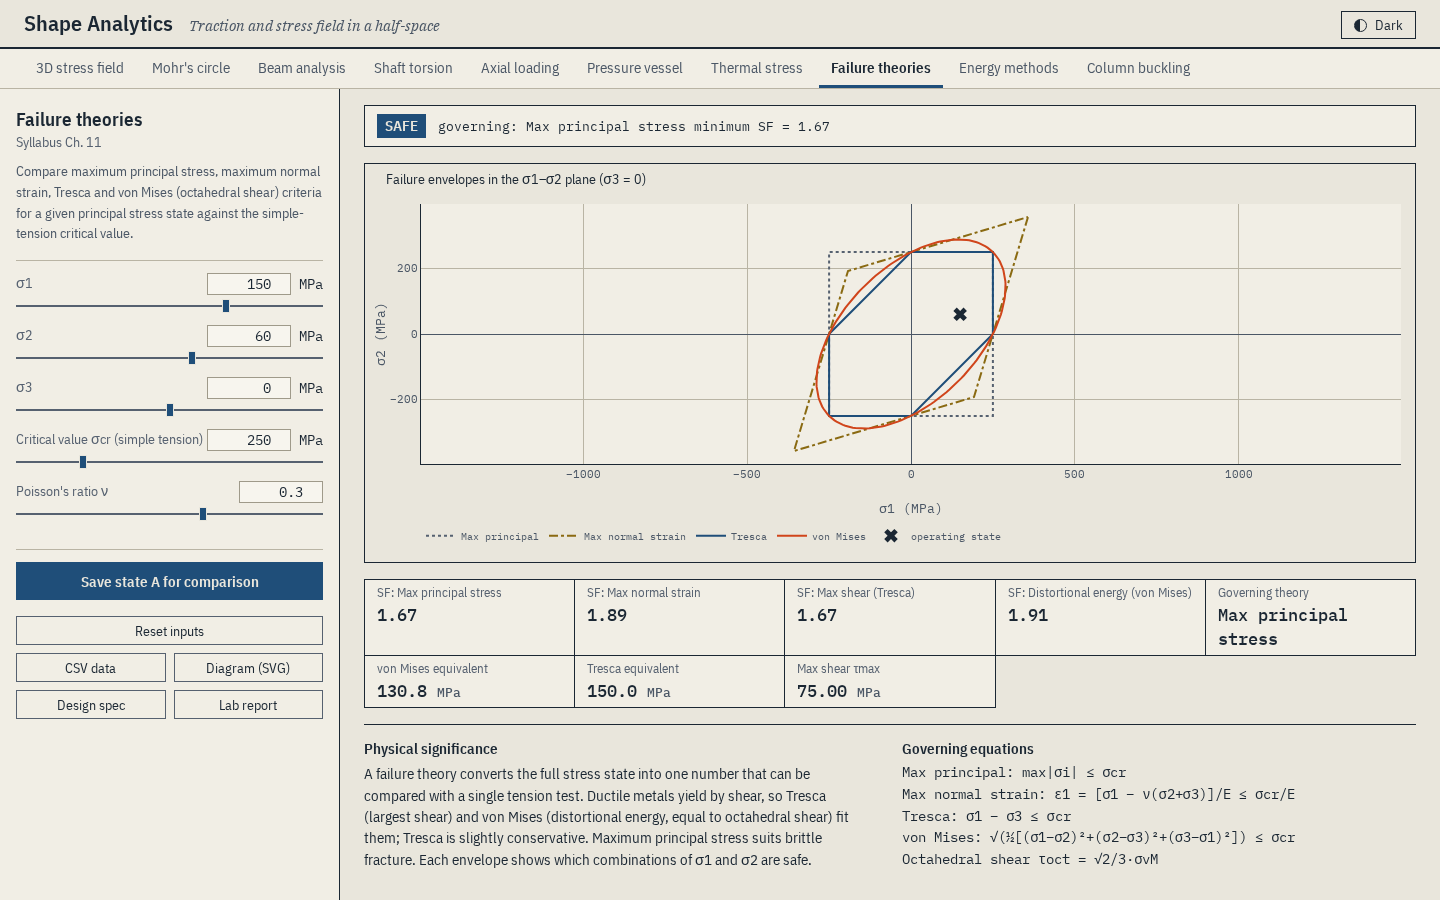
\includegraphics[width=0.95\linewidth]{figures/failure.png}
\caption{Failure theory simulator: envelopes in the $\sigma_1$--$\sigma_2$ plane and safety factors.}
\end{figure}

\section{The 3D stress field simulator}
The original module of the app combines Chapters 2 to 6 for a body loaded by a traction on an arbitrary painted area. The stress inside a half-space under a point force is given by the Boussinesq solution for a normal load and the Cerruti solution for a tangential load; both satisfy equilibrium, compatibility and the traction boundary condition. A distributed load is obtained by superposition over the painted area, which is valid because the governing equations are linear (Chapter 10, linearity and superposition). The stress tensor at each point is converted to $\sigma_n$, $\tau_{\max}$, the von Mises stress and strain magnitude using Chapters 4 to 6, and the displacement field gives the deformed shape.

\sig{The model shows how a local load spreads with depth: stress decays rapidly away from the loaded area (St.\ Venant's principle) while the volume of loaded material grows. It also demonstrates that a purely normal surface traction produces shear stress below the surface, which is where yielding can start.}

\section{Limitations}
\begin{itemize}
\item All models are linear elastic and small-strain. Plasticity (Chapter 6.8), large rotations and dynamics are not modelled.
\item Beam deflections are obtained by numerical integration on 401 points; the Timoshenko correction uses a constant shear factor.
\item The Lam\'e solution assumes a long vessel with closed ends and uniform temperature. The half-space solution is used as an approximation for a finite body in the 3D field.
\item The column simulator assumes an ideal straight, concentrically loaded column; imperfections lower the real buckling load.
\end{itemize}

\section{Verification}
The closed-form results of each simulator were checked by hand for the default case: a simply supported beam with a central load gives $M_{\max}=PL/4=7.5$~kN\,m and $\delta=PL^3/48EI=1.03$~mm; the circular shaft gives $\tau_{\max}=TR/J=32.6$~MPa and $\phi=1.17^\circ$; the plane-stress Mohr circle gives $\sigma_{1,3}=93.4,\,-33.4$~MPa; the Lam\'e hoop stress at the inner wall agrees with $pr/t$ to $0.1\%$ for $t/a=0.06$; and Castigliano's derivative of $U$ reproduces $PL^3/3EI$ for the cantilever.

\end{document}
